\chapter{Návrh a implementace}
V této kapitole bude popsán návrh backendu, který se skládá s současného návrhu, navržených změn a návrhu chybějící funkcionality. A také, bude popsána implementace navržených a změn a chybějící funkcionality podle existujícího návrhu aplikace.

Při úpravách současného návrhu byl udělán velký počet změn různé významnosti. V této kapitole budou uvedeny jenom důležité změny. Při implementaci návrhu autorovi velmi pomohlo přečteni doporučené literatury.\cite{pro-spring-boot-2}

\section{Úpravy podle požadávků}\label{navrh:upravy}
    V teto sekce budou popsány navrženy změny a jejích implementace vzhledem k nedostatkům aktuálního návrhu, které byly nalezeny během vývoje backendové a forntendové částí aplikace. 
    
    \subsection{Interval}\label{narh:upravy:interval}
        \begin{figure}\centering
	        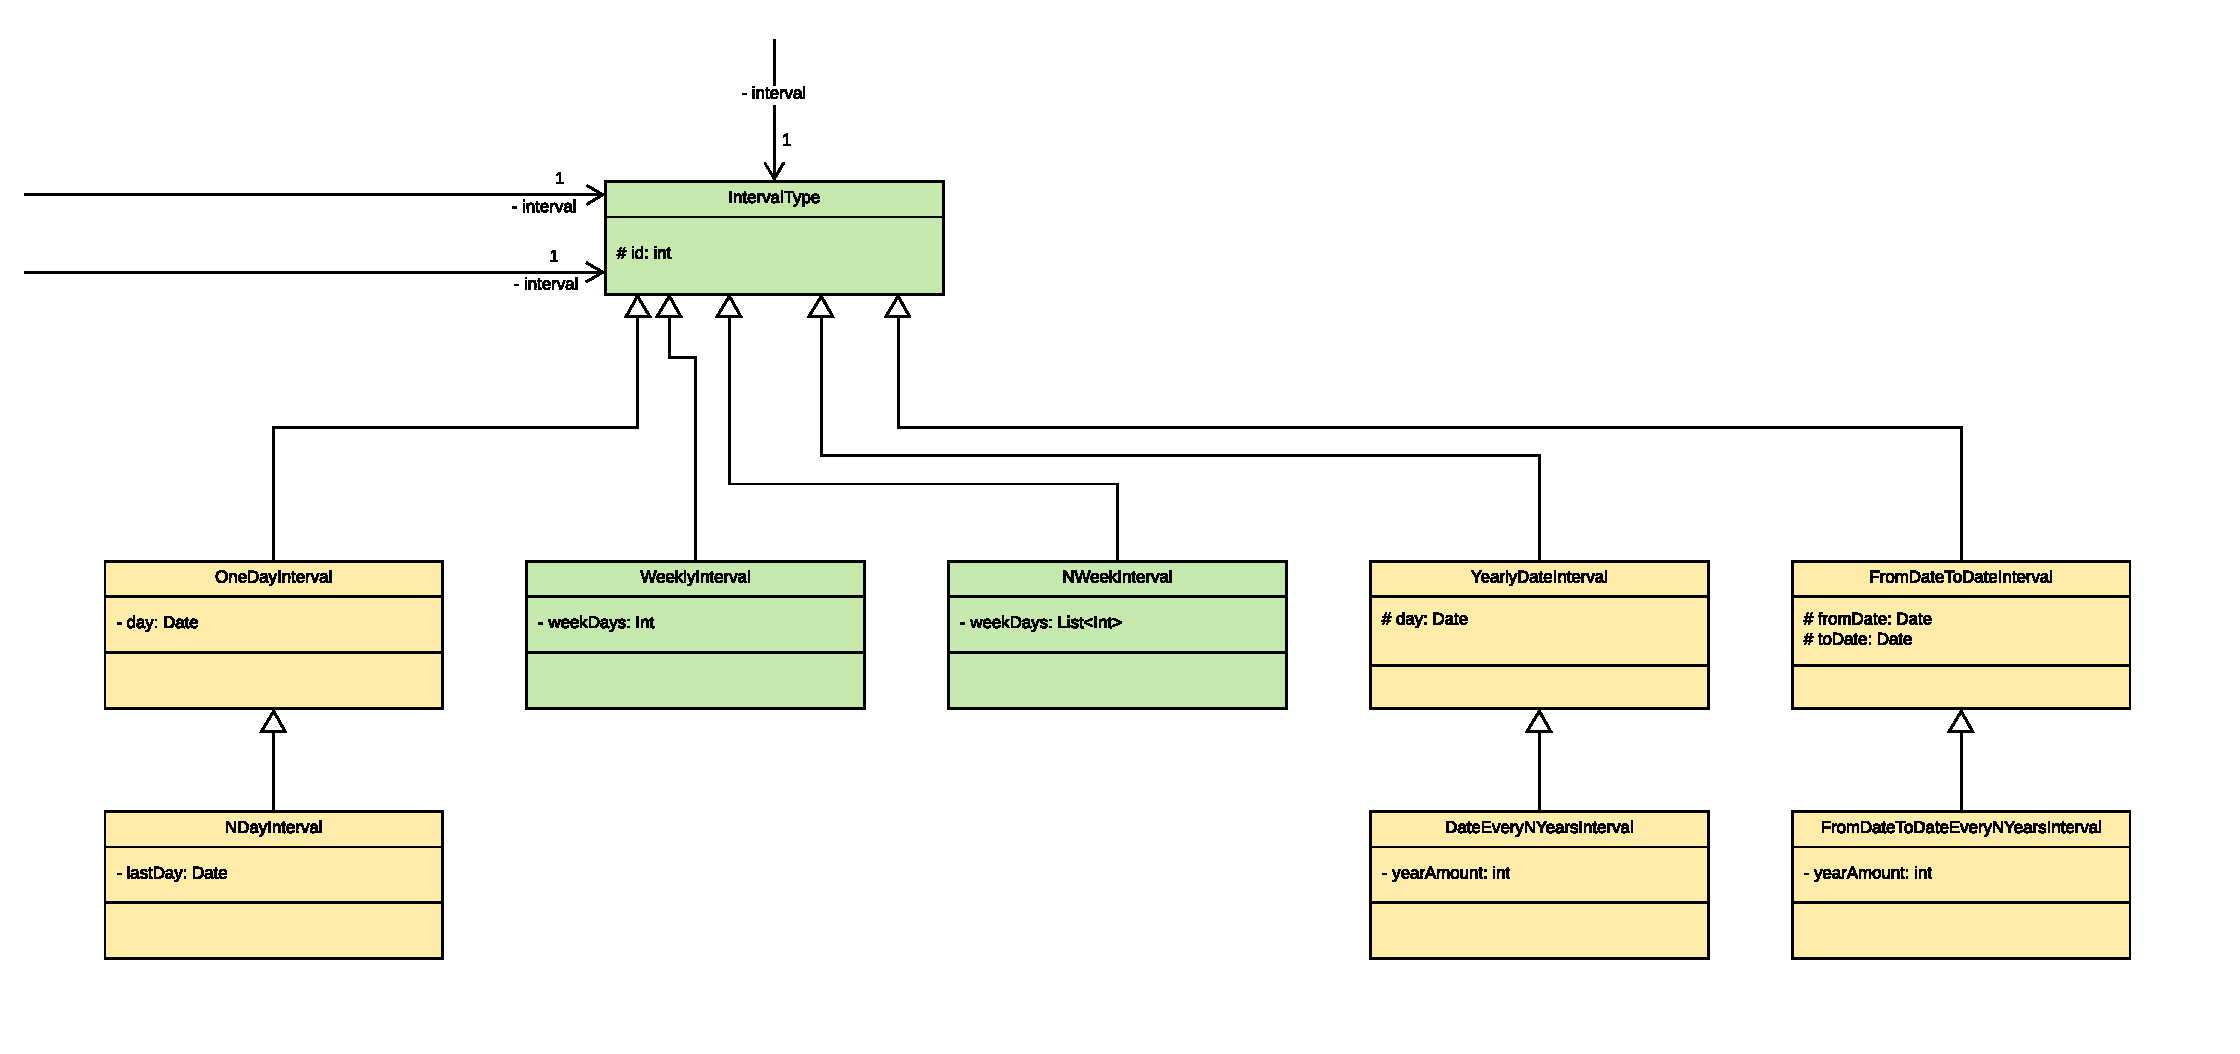
\includegraphics[width=1.0\textwidth]{pdfs/Interval1}
	        \caption[Návrh intervalu]{Návrh entity \textit{Interval} v Doménovém modelu z předmětu BI-SP2}\label{image:Interval1}
        \end{figure}
        \begin{figure}\centering
	        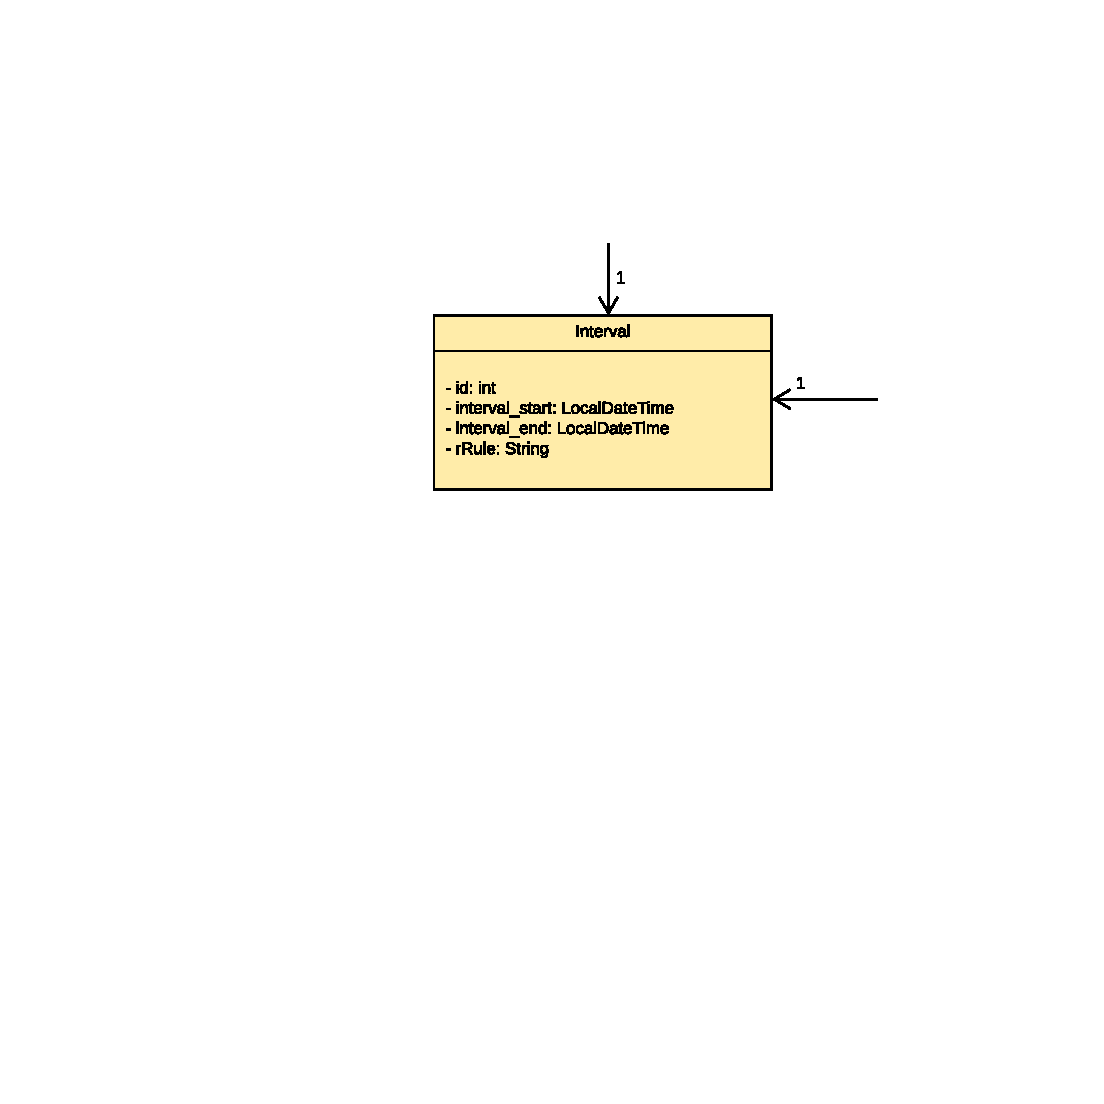
\includegraphics[width=0.5\textwidth]{pdfs/Interval2}
	        \caption[Návrh intervalu]{Nový návrh entity \textit{Interval}}\label{image:Interval2}
        \end{figure}
        \begin{figure}\centering
	        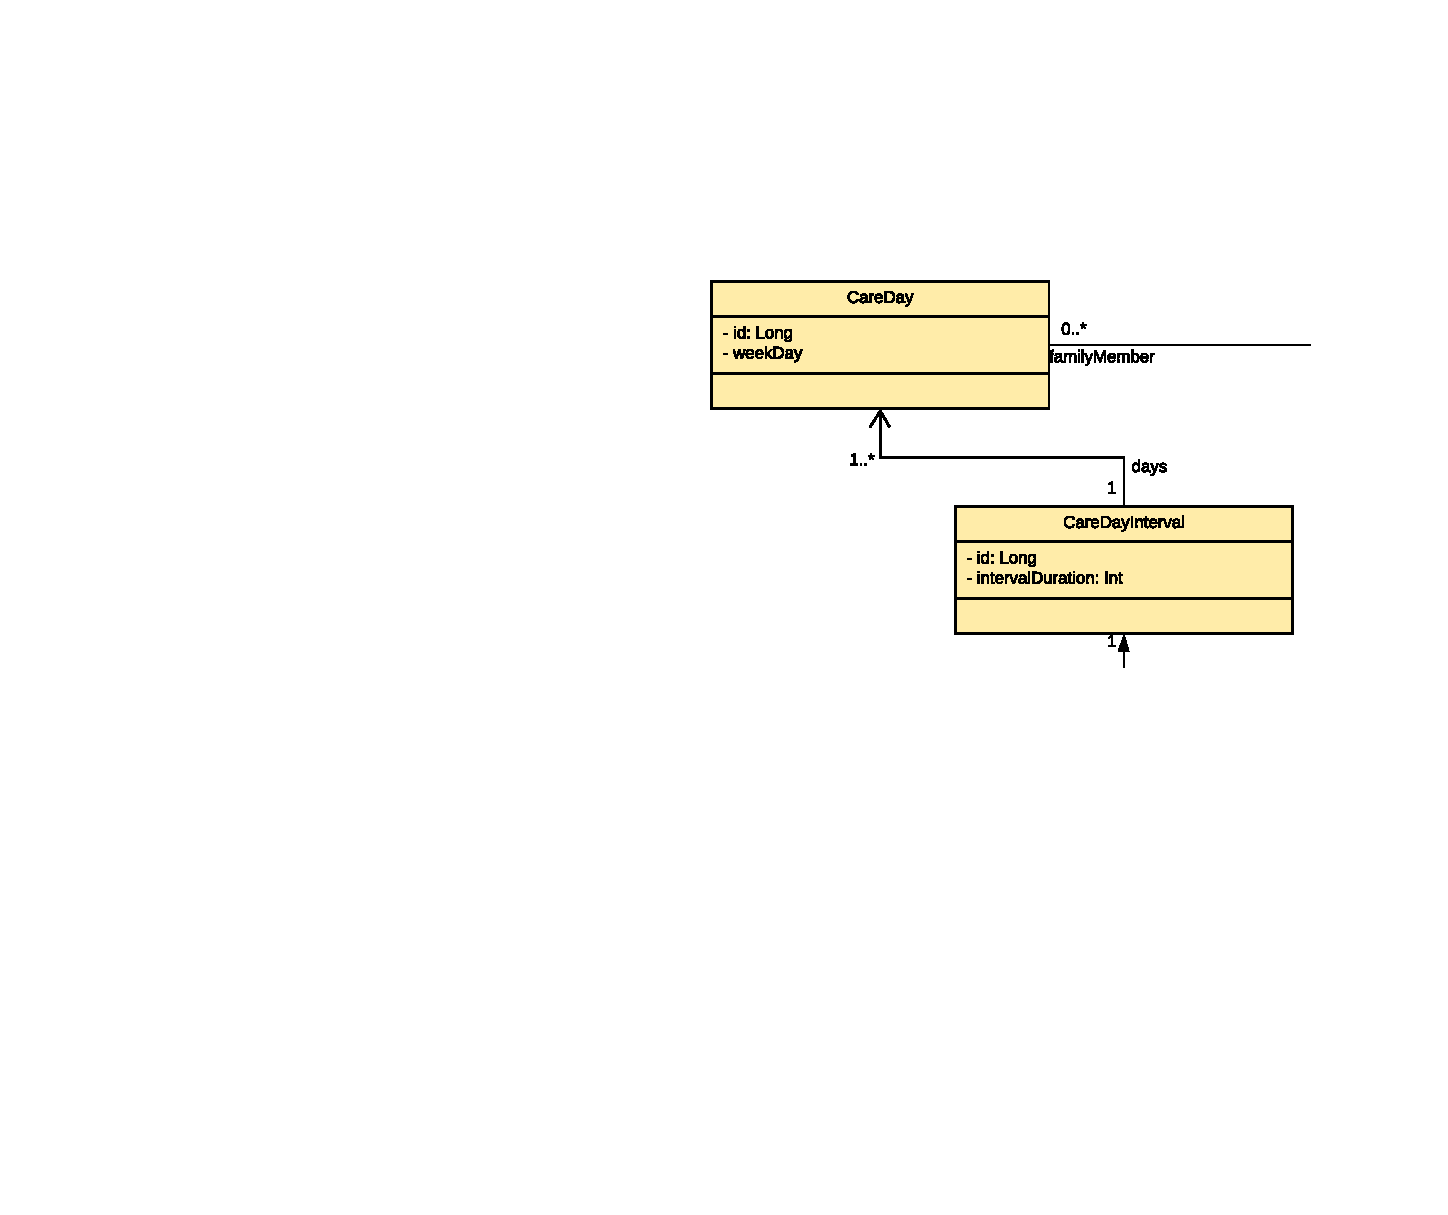
\includegraphics[width=0.5\textwidth]{pdfs/CareDayInterval}
	        \caption[Návrh intervalu]{Návrh entity \textit{CareDayInterval}}\label{image:careDayInterval}
        \end{figure}
        První změnou je nový návrh entity Interval. Původní návrh (viz. obrázek \ref{image:Interval1}) nevyhovoval svojí složitostí a zároveň jenom částečným pokrytím možných případů. Podrobněji teto problém je popsán v sekci \ref{analyza:pozadavky-frontendu}. Entita interval byla rozdělena do dvou entit. První entita (viz. obrázek \ref{image:Interval2}) úplně nahrazuje původní entitu. Druhou entitou je \textit{CareDayInterval} (viz. obrázek \ref{image:careDayInterval}), která reprezentuje časové rozmezí pečovatelských dnů.
    
        Nový návrh je postaven na úplně jiném principu. Časové rozmezí může být reprezentované dvěma způsoby. Oba dva způsoby vyžadují uvedení začátku intervalu. Tento parametr je povinný. První způsob, kromě začátku intervalu, vyžaduje i konec intervalu. Takovým způsobem můžeme definovat jednorázový interval po sobě jdoucích dnů. Druhý způsob vyžaduje zadání pravidlo opakování. Takhle můžeme definovat stejnou interval, ale mnohem složitějším způsobem. Na druhou stranu, pomocí takového pravidla můžeme definovat libovolně složitý interval. Takový návrh vyžaduje aby, buď byl zadán jenom konec intervalu, nebo bylo jenem zadáno pravidlo opakování. Pokud tyto dva parametry budou zadány najednou, server vyhodí chybu a zastaví vytvoření nesprávného intervalu.
    
        Pravidlo opakování je reprezentováno pomocí textového řetězce a má být zadáno ve standardu {RFC 5545}\cite{recurrence-rule}. Pro pohodlné testování byl navržen a implementován {interní DSL jazyk}\footnote{DSL jazyk využívající obecný programovací jazyk}, který bude popsán v sekci \ref{navrh:zmeny:dsl}.
        
    \subsection{Alimenty}\label{navrh:upravy:alimenty}
        Druha důležitá úprava současného návrhu se tyká třídy \textit{Alimony} a spravování instancí teto třídy. Podrobněji příčiny potřeby úprav byly popsány v sekci \ref{analyza:pozadavky-frontendu}. Tato sekce je věnovaná popisu navržených úprav samotných.
    
        \subsubsection{Úprava entity}
            Za účelem větší samostatnosti instancí entity \textit{Alimony} byla přidána závislost na entitu \textit{Family}. Také byl přidán atribut \textit{value}, který kopíruje stejný atribut z entity \textit{AlimonySetting}. Příčinou přidání tohoto atributu je možnost aktualizování konfigurací alimentů. V případě, že rodiče změní hodnotu alimentů, ztratí se možnost zjistit hodnoty alimentů, které byly vytvořeny do změny.
            
        \subsubsection{Spravování alimentů}
            V teto sekci bude popsán návrh třídy, která se věnuje vytváření alimentů.
        
            Všechny instance alimentů je potřeba vytvářet každý měsíc. Proto tento proces byl objednán do jednoho procesu, který je stejný pro všechny instance. Proces vytváření alimentů zajišťuje jedna metoda (viz. obrázek \ref{code:create-alimony}), která se nachází ve třídě \textit{AlimonyFactory}. Metoda vyhledáva všechny aktivní instance \textit{AlimonySetting} a pro každou vytvoří alimenty. Aktivita nastavení je zajištěna atributem \textit{enabled}, který byl přidán v rámci úprav pro rozlišování serverem aktivních a neaktivních nastavení alimentů.
            \begin{figure}
                \begin{minted}{java}
/**
*  Method generating Alimony instances based 
*   on AlimonySettings(enabled) from DB.
*
*  Scheduling is configured by the cron expression,
*  that you need to configure in application-{profile}.properties 
*   (scheduled.alimonyFactory.cronExpression).
*/
@Scheduled(cron = "\${scheduled.alimonyFactory.cronExpression}")
fun createAlimonyForEachAlimonySetting() {
    logger.info("Started scheduled alimony creation process;")
    val alimony = alimonySettingRepository
                        .findAllByEnabledTrue()
                        .map { it.createAlimony() }
    if (alimony.isNotEmpty()) {
        alimonyRepository.saveAll(alimony)
    } else {
        logger.debug(
            "AlimonyFactory didn't find any AlimonySetting to work with;"
            )
    }
}
                \end{minted}
                \caption{Ukázka metody vytvářející instance alimentů} 
                \label{code:create-alimony}
            \end{figure}
            
            Vytvářeni alimentů má být pravidelné a nemusí vyžadovat účast člověka. Proto byla využita funkcionalita frameworku Spring, která poskytuje možnost plánování automatického spouštěni. \cite{spring-scheduling}Anotace \textit{Scheduled}, která zapíná plánování pro konkretní metodu, vyžaduje \textit{cron} výraz. Tento výraz je textovou řádkou, která se skládá z čísel oddělených čárou, reprezentujících čas spouštění metod\cite{cron-expression}. Implementace byla provedena podle návody z knihy\cite{sbr:spring-task-scheduling}.
            
            \begin{figure}
                \begin{minted}{yaml}
\# Cron expression: at 01:01 AM on the 1st day of every month
scheduled.alimonyFactory.cronExpression=0 1 1 1 * ?
                \end{minted}
                \caption{Ukázka konfigurace \textit{cron} výrazu} 
                \label{code:cron-expression}
            \end{figure}
            Pro pohodlnou konfiguraci času spouštěni metody, \textit{cron} výraz byl přesunut do souboru \textit{application-{profile}.properties}, kde \textit{profile} je aktuální profilem serveru. Podrobněji návrh profilu bude popsán v sekci \ref{navrh:profily}. Pro zadání \textit{cron} výrazu je potřeba definovat \textit{property} \textit{scheduled.alimonyFactory.cronExpression} (viz. obrázek \ref{code:cron-expression}).
            
            \begin{figure}
                \begin{minted}{yaml}
scheduled.alimonyFactory=true
                \end{minted}
                \caption{Ukázka \textit{property} zapinající \textit{AlimonyFactory}} 
                \label{code:alimony-factory-true}
            \end{figure}
            Pomocí konfiguračního souboru byla přidána možnost měnit čas spouštění metody, ale také bychom potřebovali mít možnost vypnout tuto metodu. Proto přidána třída, která vytváří instanci tříd, obsahující automaticky spustitelné metody, podle \textit{property} konfiguračního souboru. V případě, že nutné \textit{property} nebyly definovány aplikace se neukončí běh a nastaví tyto \textit{property} na implicitní hodnoty. Pro zapínaní běhu metody vytvářející alimenty je potřeba definovat \textit{property} \textit{scheduled.alimonyFactory} a nastavit na hodnotu \textit{true} (viz. obrázek \ref{code:alimony-factory-true}).
        
        \subsection{Pečovatelské dny}\label{navrh:upravy:caredays}
            \begin{figure}\centering
	            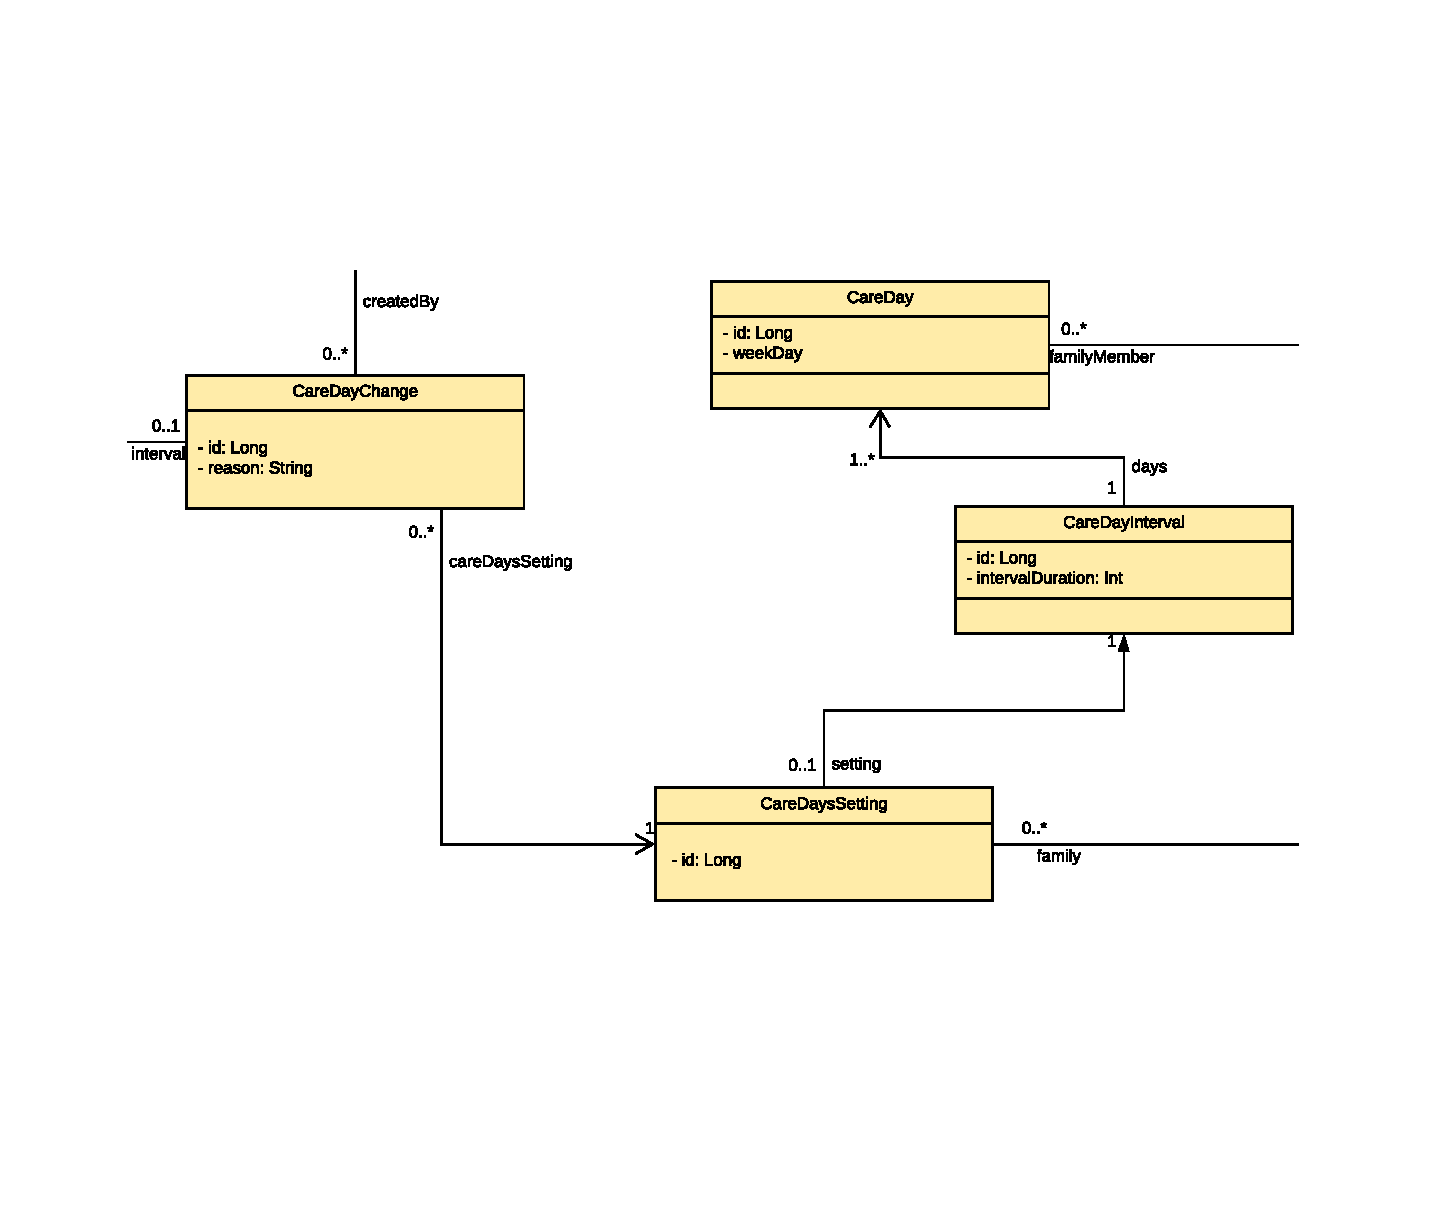
\includegraphics[width=0.8\textwidth]{pdfs/CareDays2}
	            \caption[Nový návrh pečovatelských dnů]{Nový návrh pečovatelských dnů}\label{image:caredays2}
            \end{figure}
            Podrobný popis problému byl popsán v sekci \ref{analyza:pozadavky:caredays} . Tady se soustředíme na návrhu řešení, vyhovujícím frontendové části aplikace. V předchozím návrhu implementace dlouhodobých nastavení pečovatelských dnů pro rodiče a jednorázové nastavení byly reprezentované pomocí jedné entity (viz. obrázek \ref{image:caredays1}). Kostra problému právě ve sjednocení několika problému do jednoho. Proto bylo vyřešeno řešit problém distribucí. Výsledný návrh se skládá s čtyř entit (viz. obrázek \ref{image:caredays2}):
            \begin{itemize}
                \item \textit{CareDaysSetting}, reprezentující dlouhodobé nastavení pečovatelských dnů
                \item \textit{CareDayInterval}, reprezentující interval pečovatelských dnů pro dvoudobé nastavení
                \item \textit{CareDay}, reprezentující jeden pečovatelský den pro dlouhodobé nastavení
                \item \textit{CareDayChange}, reprezentující změnu pečovatelských dnů
            \end{itemize}
            
            Dlouhodobá nastavení jsou reprezentovány seznamem pečovatelských dnů, kde každý den má odkaz na člena rodiny, který má v tento den peče o dítě. Jeden \textit{CareDayInterval} obsahuje seznám takových pečovatelských dnů, ale nereprezentuje nastavení. Za účelem pohodlné modifikovatelností, \textit{CareDayInterval} je jenom pomocnou entitou, kterou udržuje entita \textit{CareDaysSetting}, reprezentující dlouhodobé nastavení pečovatelských dnů. Tudíž, uživatel má možnost změnit interval pečovatelských dnů tím, že nahradí jiným záznamem, a současně bude vytvořena kopie tohoto záznamu v historii.
            
\section{Navržené změny}
    V teto sekci budou popsány navržené změny autorem teto práci, které vylepšují výslednou aplikaci.
    
    \subsection{Interní DSL}
        % TODO popsat podrobneji
        \begin{figure} % [H] TODO
            \begin{minted}{java}
/**
* Valid Interval with recurrence rule.
*/
private val validInterval = Interval(
        id = 1,
        interval_start = creationTime,
        interval_end = null,
        rRule = rule(frequency = Frequency.WEEKLY, count = 10) {
            byDays {
                and(DayOfWeek.MONDAY)
                and(DayOfWeek.WEDNESDAY)
                and(DayOfWeek.SUNDAY)
            }
        }
)
            \end{minted}
            \caption{Ukázka \textit{Intervalu} s pravidlem opakování} 
            \label{code:valid-interval}
        \end{figure}
        Pro pohodlné testování byl implementován interní DSL jazyk poskytující možnost vytvořit pravidlo opakovaní. Dále uvádím příklad \textit{Intervalu}, který má pravidlo opakování vytvořené pomoci DSL jazyku. Tento interval bude použit při testování.

    \subsection{Album}
        TODO
        
    \subsection{Oznámení}
        TODO alert a notification
        
    \subsection{Konverter}
        TODO popis konverteru mezi entitou i dto
        
    \subsection{Našeptavač pro výjimky}
        TODO novy format vyjimek + pridane nove vyjimky
        
    \subsection{Implementace servisní vrstva}%prejmenovat na ceskou verzi
        TODO business logika ohledne updatovani a vytvoreni entit
        
    \subsection{Implementace Controlleru}
        TODO POST vs PUT
    
    \subsection{Implementace historie změn}
        Důležitou častí aplikace je zaznamenání změn udělaných uživatelem. Úpravou je změna záznamu entity, kterou uživatel s rolí \enquote{ROLE\_USER} může upravit. Aktivita \textit{root}\footnote{uživatel s rolí \enquote{ROLE\_ROOT}} uživatel není zajímavá, protože tento uživatel je odstraněn v rámci profilu pro produkci. Příkladem takové změny může být změna nastavení alimentů nebo označení oznámení jako přečtený.
    
        \begin{figure}\centering
	        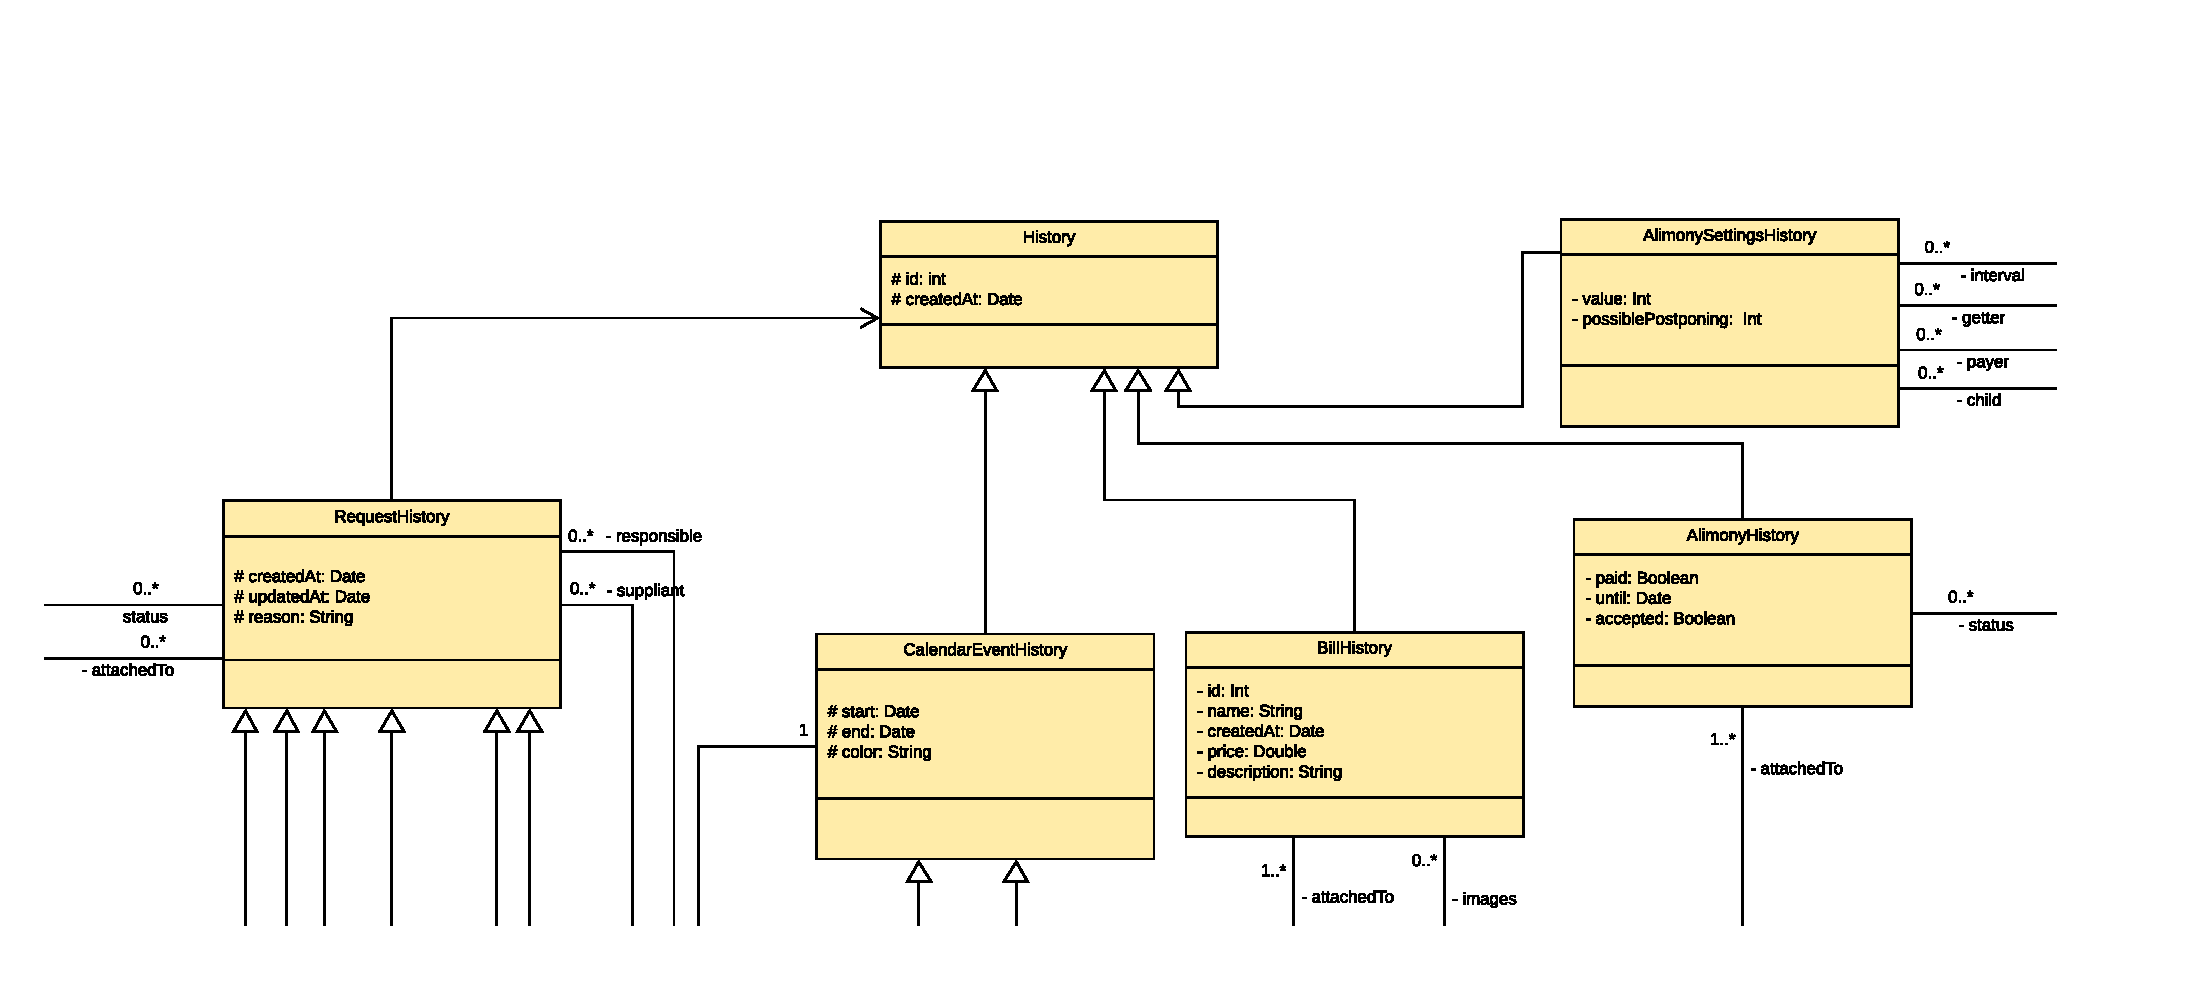
\includegraphics[width=1.0\textwidth]{pdfs/History1}
	        \caption[Návrh entity History]{Návrh entity \textit{History} podle Doménového modelu z předmětu BI-SP2}\label{image:History1}
        \end{figure}
        Historie změn ještě nebyly implementovány, ale návrh již existoval a hlavní myšlenka se zůstává úplně stejnou. Záznam historie kopíruje všechny atributy entity a přidává čas vytvoření záznamu a vlastní identifikátor\footnote{identifikátor v rámci databáze}. Entita History je abstraktní třídou, neboli generalizace v případě návrhu v doménovém modelu. Jednotlivé entity, které jsou zděděné od teto entity, reprezentuje historie příslušné entity (viz. obrázek \ref{image:History1}). 
    
        \begin{figure}\centering
	        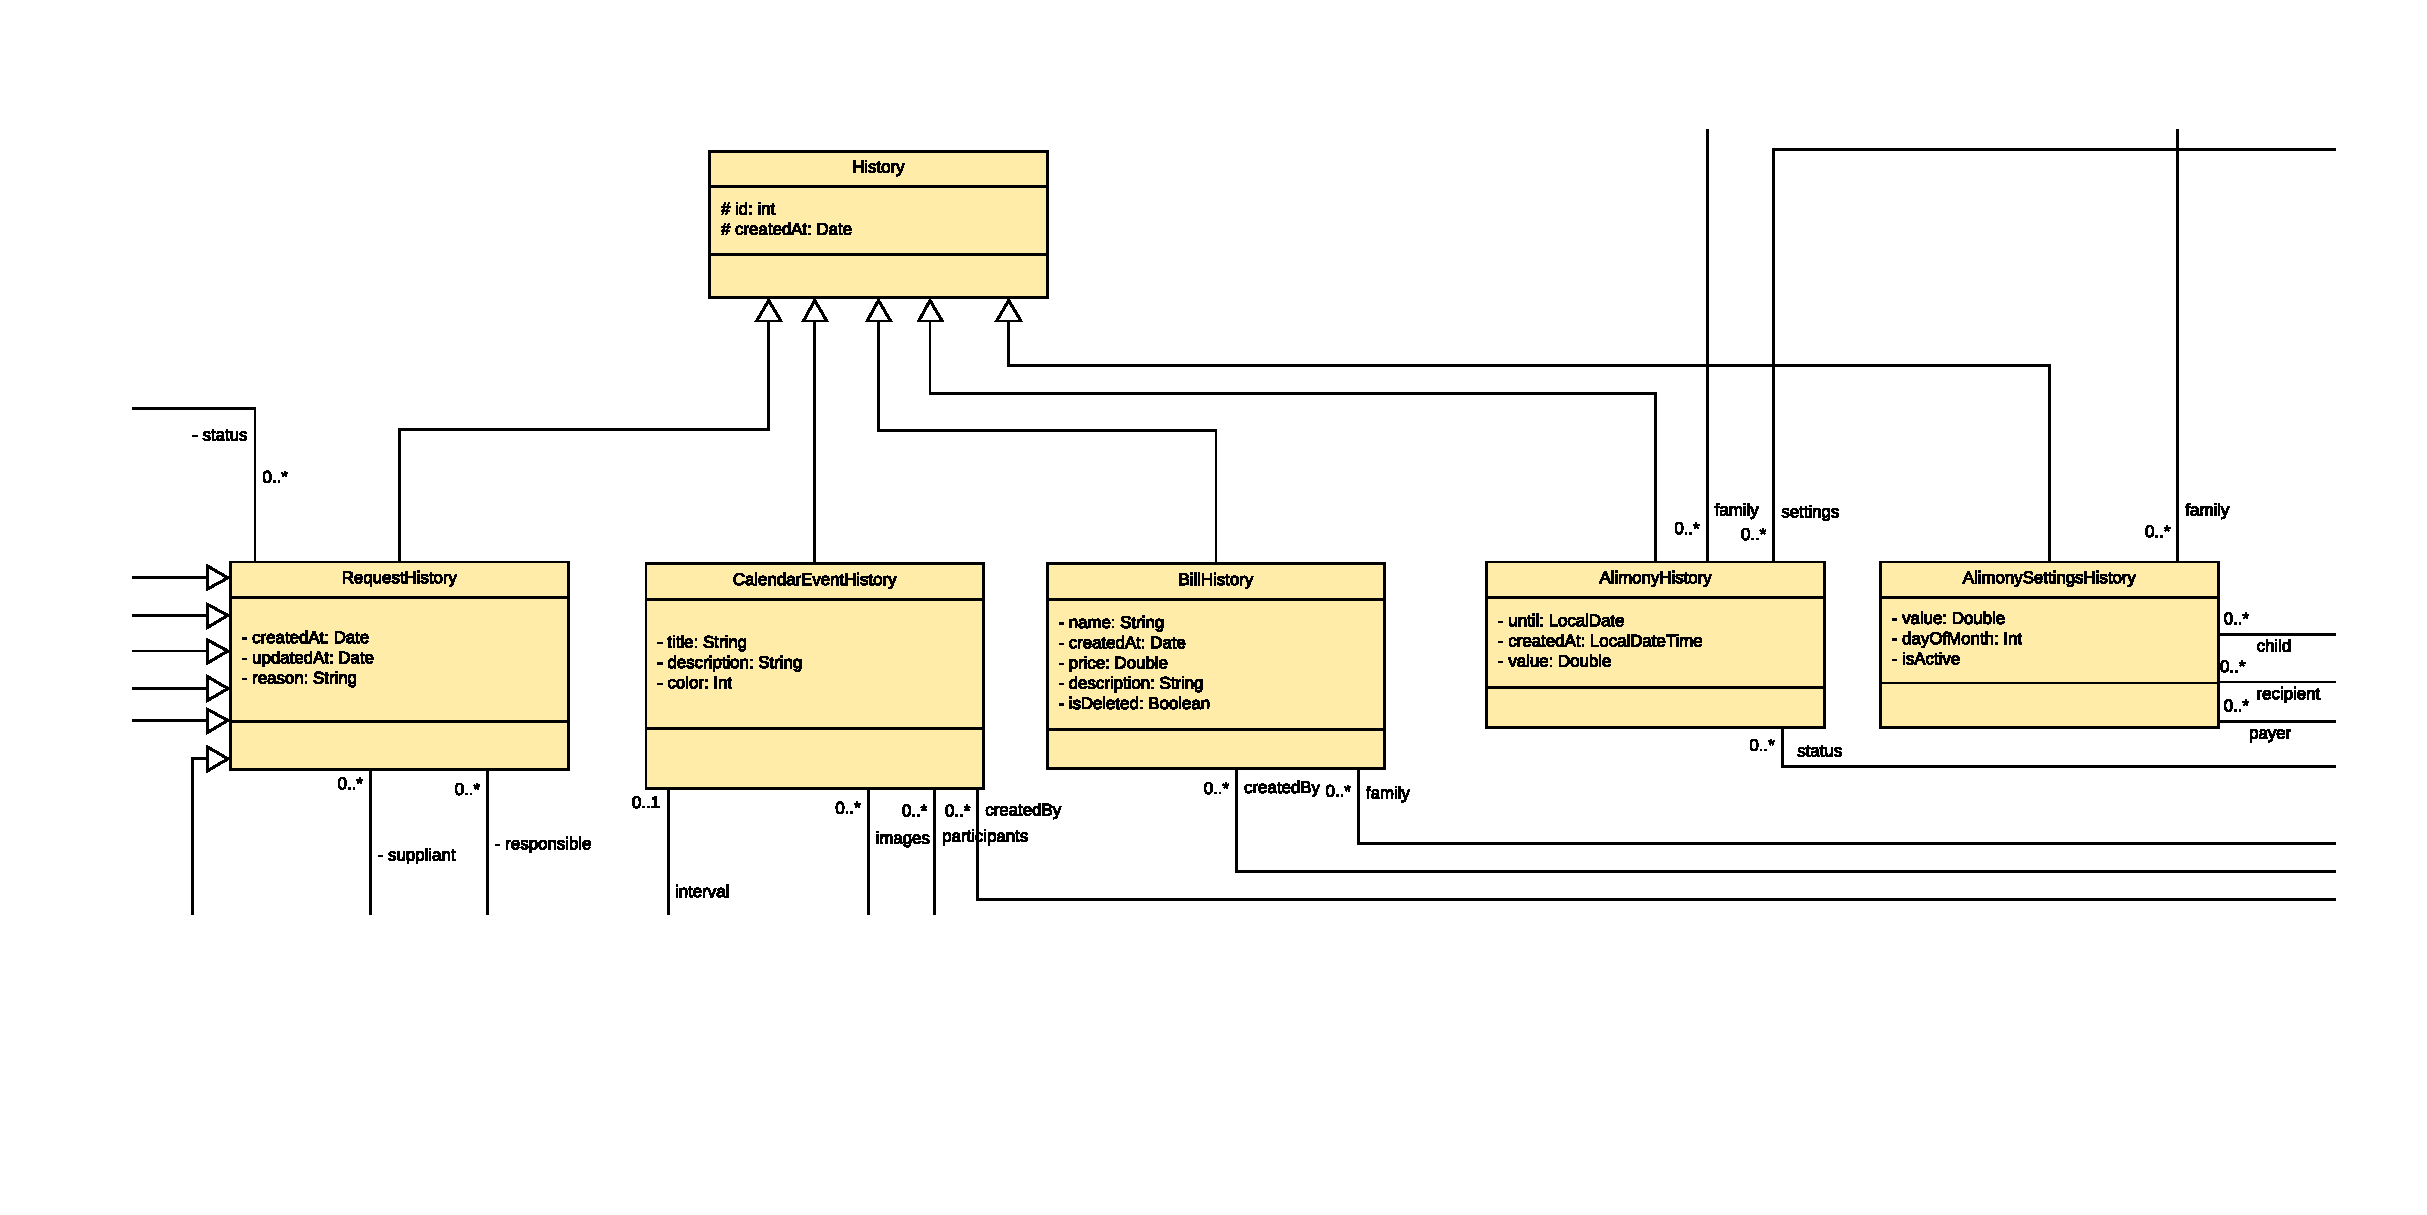
\includegraphics[width=1.0\textwidth]{pdfs/History1_2}
	        \caption[Návrh entity History po změnách návrhu]{Návrh entity \textit{History} po navržení změn pro entity, kterým patří příslušné entity historie}\label{image:History1_2}
        \end{figure}
        Tato entita byla implementována jako poslední a všechny změny, které se ji týkají, jsou srozumitelné jenom po přečtení všech změn návrhu. Než se zanořit do navržení vhodných změn teto entity, byla potřeba nejdřív upravit návrh podle navržených změn (viz. obrázek \ref{image:History1_2}). Byly opraveny atributy, které mají entity v souladu s entity, kterým patří jednotlivé historie.
        
        Dalším krokem úprav je navržení úprav, které už není nutné, ale výrazně zlepšují výsledný návrh serveru:
        \begin{itemize}
            \item přidání do každé entity History odkazů na příslušnou entitu. Například, entita AlimonyHistory bude mít navíc odkaz na entitu Alimony.
            \item zavedení nové entity CareDaysSettingHistory podle návrhu entity CareDaysSetting, která byla popsána v sekci \ref{navrh:upravy:caredays}
        \end{itemize}
         TODO image
        Výsledný návrh entity History (viz. obrázek \ref{image:History2}) byl kompletně implementován a provázán s funkcionalitou příslušných controllerů. Implementace vyžadovala rozdělení servisní vrstvy do dvou logických bloků. První blok se zabývá spravováním požadavků frontendové části aplikace, což aktuálně jsou požadavky na nalezení všech existujících záznamu a požadavky na nalezení konkretního záznamu podle jejího identifikátoru. Historii změn by neměl spravovat uživatel, proto byl mazání, upravování a mazání záznamu těchto entit jsou zakázány pro uživatele. Celou logikou se zabývá server samotný. Za tímto účelem byl vytvořen druhý logický blok servisní vrstvy, který poskytuje možnost vytvořit konkretní historii. Typ historii, který bude vytvořen definuje typ DTO, který předán do metody.

\section{Návrh bezpečnosti}\label{navrh:bezpecnost}
    \subsection{OAuth 2.0}
        % TODO
        TODO Za účelem zabezpečení procesu autorizace byl zvolen protokol OAuth 2.0 . 
        
    \subsection{HTTPS}
        certificaty TODO
        
\section{Návrh požadavků na změny}\label{navrh:requests}
    TODO bude v budoucích krocích
        
\section{Profily}\label{navrh:profily}
    Při implementace byl rozšířen návrh profilů aplikace. Původní návrh obsahoval jenom implicitní profil a vývojový profil, dosahující konfiguraci databáze H2. Výsledný návrh aplikace potřebuje více profilu, proto byly přidány dva profily aplikace: profil pro produkce a profil pro testování. Příčinami přidání dalších profilu jsou rozdíly mezi konfiguracemi, která potřebují konkretní případy spouštěni aplikace. Princip chovaní profilu byl již zmíněn v sekci \ref{analyza:soucasnaImplementace:profily}, proto ihned se zanoříme do provedených změn.
    
    Pro podrobnější popis přidaných profilu je potřeba nejdříve popsat výslednou konfigurací existujícího profilu pro proces vývoje. Dále uvádím seznam provedených změn a rozšíření, které se navazují na tento profil:
    \begin{itemize}
            \item Rozšířeni konfigurace databáze. Změny byly provedeny za účelem přesnější definici konfiguraci \ref{navrh:db} . 
            \item Přidáni vyžadováné konfiguraci pro bezpečnost aplikace, která byla popsána v sekci \ref{navrh:bezpecnost} 
            \item Přidaní proměnné do konfiguraci, která zapíná AlimonyFactory (viz. sekci \ref{navrh:upravy:alimenty}) a zároveň proměnné definující pravidlo, podle kterého se řídí plánováni spouštění této třídy.
            \item Přidání závislostí implementace userDetails, která má implicitního uživatele s roli \enquote{ROLE\_ROOT} (viz. sekci \ref{navrh:bezpecnost})
            \item Přejmenování profilu s \enquote{development} na \enquote{dev}, za účelem lepší elegance kódu při definování několika profilu třídy najednou.
    \end{itemize}
    
    Výše uvedena konfigurace je vhodná pro vývoj aplikace, ale zároveň není vhodná pro produkci a testování aplikace, proto vyřešeno nechat v implicitní konfiguračním souboru jenom uvedení profilu, který by měla aplikace využit pro následující spuštění aplikace.
    
    Prvním profilem, který byl přidán, je profil pro produkci. Hlavním rozdílem tohoto profilu od profilu vývoje je využita databáze. Podrobněji zvolená databáze podle popsána sekce \ref{navrh:db}. Pro tuto sekci je postačující zmínit, že zvolena databáze byla PostrgesSQl, což je odlišná databáze od H2, která je využita pro testování. Druhou odlišností je jiná implementace UserDetails. Produkční verze aplikace by neměla mít \textit{root} uživatele, který má přistup do libovolné metody. Jiný konfigurační soubor také dovoluje nechat konfiguraci pro produkci nedotčenou při možném velkém počtu změn v jiných profilech.
    
    Druhým profilem, který byl přidán do aplikace je profil pro testování. Změny se dotýkají stejných aspektu jako i profilu pro produkci. Byla přidána nova implementace rozhraní UserDetails, která obsahuje implicitních uživatelů s různými roli pro pohodlné testování  Také byla přidána konfigurace databáze, která je zatím stejná jako u profilu pro vývoj, ale bylo definováno chování databáze jako \textit{create-update}. Při definováni jiného chování databáze můžou vyskytnout problémy při spouštění integračních testů.
    
\section{Databáze} \label{navrh:db}
    Popis používané databáze už vyskytoval v rešerši (viz. sekci \ref{resere:databaze}) a analýze (viz. sekci \ref{analyza:soucasnaImplementace:databaze}), proto tady jenom zmíním, že se používá relační databáze H2. Pro popis zvolených databází pro proces realizace praktické části je potřeba zmínit, že aplikace byla rozdělena do různých profilů. Používána databáze je jedním z rozdílů těchto profilů. Podrobněji profily aplikace byly popsány v sekci \ref{navrh:profily} .
    
    Profily pro vývoj a testováni používají databázi H2. Stejná databáze byla použita při předchozí implementaci a nevyžadovala její nahrazeni jinou databází. Zdroj databáze byl změněn z konkretního souboru na paměť aplikace, což znamená, že databáze se vytváří při každém spouštění aplikace a zničí se po její ukončení. Také byl definován konkretní dialekt databáze. Byl zvolen implicitní dialekt, který poskytuje databáze H2, protože zvolená databáze pro produkci.
    
    Pro profil produkce bylo vyřešeno použit jinou databází. Byly zvoleny dva kandidáty: PostgresSQL a MySQL. Tyto databáze jsou jedeními z nepopulárnějších databázi na moment napsáni teto bakalářské práci a zároveň jsou otevřeným softwarem.
    
    % TODO popsat podroneji kazdou databazi a pak napsat vysledek proc jedna byla vybrana
    Obě dvě databáze jsou skvěle, ale, po porovnání těchto dvou databázi, výslednou databází byla zvolena databáze PostgresSQL. Některá funkcionalita byla považovaná za důležitou i když není ještě využita v implementaci a návrhu.
    \begin{itemize}
            \item PostgresSQL je objektově relační databáze\cite{postgres-about}, kdy MySQL je jenom relační databáze\cite{mysql-wiki}. Tohle znamená, že PostgresSQL dovoluje dědění tabulek a přetěžování metod. MySQL takově možnosti neposkytuje.
            \item PostgresSQL poskytuje možnost definovat vlastní typy\cite{pstgres-create-type}
            \item autor teto práce má zkušenosti s PostgresSQL
    \end{itemize}
    Informace o rozdílech těchto databází byly převzaty s několika článku na internetu. Nejpoužitelnějšími pro autora teto práce byly \cite{mysql-postgres1, mysql-postgres2}
    
\section{Implementace požadavků na změny}\label{impl:requests}
    TODO requests
    
\section{Návrh testování}\label{navrh:testovani}
    Pro testování kódu budou využity frameworky JUnit 5 a Spring. Podrobný popis těchto frameworků byl v sekci \ref{resere:testovani}. Testování se skládá s \textit{unit}\footnote{testy, zaměřené na ověření správnosti fungování samostatně testovatelné části programu} testů a \textit{integration}\footnote{testy, zaměřené na ověření správné komunikace mezi komponentami} testů. Návrh testů se bude podstatné lišit mezi sebou. Proto bude využita funkcionalita frameworku JUnit 5, který od verze 5 poskytuje možnost označovat testy pomocí tagů\cite{junit-tags}. Princip chování tagů najdete v sekci \ref{resere:testovani}. Podrobnější informaci o implementaci tagů bude popsána v sekci \ref{testovani:tagy}. 
    Kompletní implementáce testování bude popsána v kapitole \ref{testovani}.
    
    \subsection{Unit testy}
        Unit testy využívají jenom funkcionalitu frameworku JUnit 5 a testují základní funkcionalitu. Otestovány mají byt třídy a metody, které mohou být otestovány samostatně. Také, tyto testy mají být označeny jako unit testy pomocí tagů.  %TODO popsat podrobneji
        
    \subsection{Integráční testy}
        Integrační testy budou testovat jednotlivé Controllery. Tyto testy jsou navrženy pomocí principu IoC\footnote{princip, za kterého kontrola nad vytvořením a provázáním tříd vlastní framework}, proto budou označeny jako integrační testy a zároveň jako pomalé testy.